\documentclass[10pt,a4paper,twocolumn]{article}

\usepackage[T1]{fontenc}
\usepackage{newtxtext,newtxmath}   % Times, like the ACM/SIGPLAN papers
\usepackage[top=1.6cm,bottom=1.6cm,left=1.7cm,right=1.7cm]{geometry}
\usepackage{enumitem}
\usepackage{titlesec}
\usepackage{booktabs}
\usepackage{array}
\usepackage[table]{xcolor}
\usepackage{tikz}
\usetikzlibrary{arrows.meta,positioning}
\usepackage[most]{tcolorbox}
\usepackage[hidelinks]{hyperref}

% One accent colour used for headings, the key formula and the diagram
\definecolor{accent}{RGB}{0,92,158}
\colorlet{accentbg}{accent!7}
\newtcolorbox{keybox}{colback=accentbg,colframe=accent,boxrule=0pt,
  leftrule=2pt,arc=0pt,left=4pt,right=4pt,top=0pt,bottom=0pt,
  boxsep=2pt,before skip=4pt,after skip=4pt}
\newtcolorbox{codebox}{colback=black!5,colframe=black!5,arc=1pt,
  left=3pt,right=3pt,top=0pt,bottom=0pt,boxsep=1pt,
  before skip=2pt,after skip=3pt,fontupper=\footnotesize}
% Circled step number, reused in the diagram and in Section 4
\newcommand{\step}[1]{\tikz[baseline=(c.base)]\node[circle,fill=accent,
  text=white,inner sep=0.8pt,font=\scriptsize\bfseries](c){#1};}

% Paper-like layout: indented paragraphs, no column rule
\setlength{\parindent}{1em}
\setlength{\parskip}{0pt}
\setlength{\columnsep}{0.8cm}
\setlength{\columnseprule}{0pt}
\setlist[itemize]{leftmargin=*,nosep,topsep=1pt,before=\raggedright}
\setlist[enumerate]{leftmargin=*,nosep,topsep=1pt,before=\raggedright}
\titleformat{\section}{\large\bfseries\color{accent}}{}{0pt}{}
\titlespacing*{\section}{0pt}{11pt}{4pt}
\newcommand{\head}[1]{\textbf{\color{accent}#1}\quad}   % run-in heading, like "Goal" in the paper
\pagestyle{empty}
\raggedbottom   % don't stretch a column's spacing to fill it

% Body text slightly below 10pt (no standard class option for this)
\makeatletter
\renewcommand\normalsize{\@setfontsize\normalsize{9.4}{11.2}%
  \abovedisplayskip 10\p@ \@plus2\p@ \@minus5\p@
  \abovedisplayshortskip \z@ \@plus3\p@
  \belowdisplayskip \abovedisplayskip
  \belowdisplayshortskip 6\p@ \@plus3\p@ \@minus3\p@
  \let\@listi\@listI}
\makeatother

\begin{document}

\twocolumn[{%
\begin{center}
    {\Large\bfseries CSPLib 068: Traveling Tournament with Flexible Hosts and Budgets}\\[8pt]
    {\large Group 16\quad$\cdot$\quad Martim Borges, David Santos}
\end{center}
\vspace{-4pt}
{\color{accent}\rule{\textwidth}{0.8pt}}
\vspace{4pt}
}]

% ------------------------------------------------------------------
\section*{1. CSPLib Problem}

\textbf{Traveling Tournament Problem with Predefined Venues}. A compact single round robin: every team plays every
other team once, one game per round, at a predefined venue, with at
most 3 home or 3 away games in a row. The goal is to minimise total
travel distance.

% ------------------------------------------------------------------
\section*{2. Our Extension: Before vs Now}

\begin{center}
\small
\renewcommand{\arraystretch}{1.25}
\begin{tabular}{@{}ll>{\columncolor{accentbg}}l@{}}
\toprule
 & \textbf{Original} & \textbf{\color{accent}Our extension} \\
\midrule
Hosts & all fixed & some flexible (\texttt{UND}) \\
Home/away & not enforced & each team hosts $\approx$ half \\
Stadiums & always open & can be closed in a round \\
Distances & circular & any symmetric matrix \\
Travel cost & -- & $E_i = c_i D_i$ \\
Budget & no limit & $E_i \le B_i$ \\
Objective & total distance & weighted distance \\
\bottomrule
\end{tabular}
\end{center}

Each team $i$ travels a total distance $D_i$, pays $c_i$ per travel unit 
and has a budget $B_i$, so its cost is $E_i = c_i D_i \le B_i$.
Fixed venues are always respected, in a flexible game the solver
chooses the host.

\head{Travel}Each team starts at home, travels directly between
consecutive away games, and returns home after the last round.

\head{Objective}The more a team's travel cost weighs on
its budget, the more its distance should count. We measure this with
the ratio $r_i = c_i/B_i$ and give team $i$ the weight
\begin{keybox}
\vspace{-8pt}
\[
w_i = 1 + \frac{r_i}{\bar r},
\qquad \bar r = \frac{1}{n}\sum_{j} r_j,
\qquad \min \sum_{i} w_i D_i .
\]
\vspace{-12pt}
\end{keybox}
\noindent The weights depend only on the input, not on the schedule. Equivalently,
the objective is the total distance plus a penalty on the share of each
budget spent. It is one objective for the whole league, not a fairness model.

% ------------------------------------------------------------------
\section*{3. Model}

The solver decides only two things: \texttt{opponent[i,k]}, the team
that $i$ plays in round $k$, and the host of each pair. The constraints are:
\begin{center}
\small
\renewcommand{\arraystretch}{1.0}
\begin{tabular}{@{}>{\bfseries}p{1.9cm}>{\raggedright\arraybackslash}p{5.9cm}@{}}
\toprule
Round robin & Symmetric pairing, \texttt{alldifferent} per team and
per round. \\\addlinespace[2pt]
Venues & $i$ is home in round $k$ iff
\texttt{host[i,opponent[i,k]] = i}. \\\addlinespace[2pt]
Streaks & At most 3 home or 3 away in a row (\texttt{regular}, 7
states). \\\addlinespace[2pt]
Balance & Each team hosts half of its $n-1$ games, rounded down or
up. \\\addlinespace[2pt]
Availability & A closed stadium cannot host that round. \\\addlinespace[2pt]
Budget & $E_i = c_i D_i \le B_i$ for every team. \\\addlinespace[2pt]
Validation & \texttt{assert}s reject invalid instances. \\
\bottomrule
\end{tabular}
\end{center}
% Sentence + diagram in one box so they never split across columns
\noindent\begin{minipage}{\columnwidth}
Everything else \emph{follows} from these by propagation:

\vspace{3pt}
{\centering
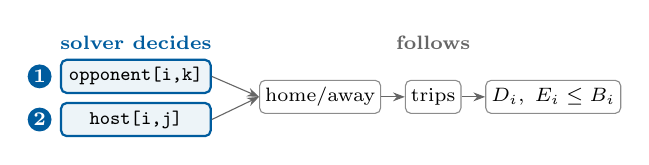
\begin{tikzpicture}[font=\scriptsize, node distance=3mm,
  dec/.style={draw=accent,fill=accentbg,thick,rounded corners=2pt,
    inner sep=2pt,minimum height=4.2mm,minimum width=19mm,
    font=\scriptsize\ttfamily},
  der/.style={draw=black!45,rounded corners=2pt,inner sep=2pt,
    minimum height=4.2mm},
  num/.style={circle,fill=accent,text=white,inner sep=0.8pt,
    font=\scriptsize\bfseries},
  arr/.style={-{Stealth[length=1.5mm]},black!60}]
  \node[dec] (opp) {opponent[i,k]};
  \node[dec,below=1mm of opp] (host) {host[i,j]};
  \node[num,left=1mm of opp] {1};
  \node[num,left=1mm of host] {2};
  \node[der,right=6mm of opp.east,anchor=west,yshift=-2.6mm] (ha)
    {home/away};
  \node[der,right=of ha] (trip) {trips};
  \node[der,right=of trip] (cost) {$D_i,\;E_i \le B_i$};
  \draw[arr] (opp.east) -- (ha.west);
  \draw[arr] (host.east) -- (ha.west);
  \draw[arr] (ha) -- (trip);
  \draw[arr] (trip) -- (cost);
  \node[above=0pt of opp,text=accent,font=\scriptsize\bfseries]
    {solver decides};
  \node[text=black!60,font=\scriptsize\bfseries] at (trip |- opp.north)
    [anchor=south] {follows};
\end{tikzpicture}\par}
\end{minipage}

% ------------------------------------------------------------------
\section*{4. Search Strategy}

\head{What we changed}The CSPLib model has no search instruction, so
the solver picks the order in which to try values. We added one
(\texttt{seq\_search}) that tells it what to decide, and in which order
(the two decisions in the Section 3 diagram):
\begin{itemize}[label={},leftmargin=1.2em,itemindent=-1.2em,topsep=3pt]
    \item \step{1}\ \textbf{Who plays whom.} Fill \texttt{opponent[i,k]}, always
    the slot with the fewest possible opponents left
    (\texttt{first\_fail}). Filling the hardest slots first exposes bad
    choices early, before much work is wasted on them.
    \item \step{2}\ \textbf{Who hosts the flexible games.} Only then pick which
    of the two teams hosts each flexible pair (\texttt{matchHost}, in
    list order). Fixed games already
    have their host.
\end{itemize}

\vspace{3pt}
\head{Why it is better}Only these two things are real choices, and
the solver finds dead ends sooner when it settles the schedule first.
The order changes speed only, not the valid schedules or the optimal
value.

% ------------------------------------------------------------------
\section*{5. Limitations}

\begin{itemize}
    \item \textbf{Big numbers.} Large budgets that are not multiples
    of each other (e.g.\ 997, 1009, 1013) make the weights used by the
    solver very large, which can overflow or slow it.
    \item \textbf{Time limit.} Bigger leagues can hit the 60 s limit,
    we then report the best schedule found, not a proven optimum.
    \item \textbf{No schedule.} Tight budgets or closed stadiums can
    make a league impossible, the program says so.
\end{itemize}

% ------------------------------------------------------------------
\section*{6. How to Run}

Tested with Python 3.14.7 and 3.12.0, MiniZinc 2.10.1 and Gecode 6.4.0.

\begin{itemize}[topsep=3pt,itemsep=6pt]
    \item \textbf{Python script} (input file):
\begin{codebox}
\begin{verbatim}
python3 proj.py <input file>
\end{verbatim}
\end{codebox}
    \item \textbf{MiniZinc model}:
\begin{codebox}
\begin{verbatim}
minizinc --solver gecode \
  TTPFVHBTDMBSA-BA.mzn instances/<name>.dzn
\end{verbatim}
\end{codebox}
\end{itemize}

% ------------------------------------------------------------------
\section*{7. Video}

% TODO: replace with \url{https://...} once the video is uploaded
[video link]

% ------------------------------------------------------------------
\section*{8. Web Resources and Generative AI Usage}

\textbf{Web resources.} [list the sites and documentation you used]

% TODO(human): 2-4 sentences in your own words: which tool, what it was
% used for (incl. this report's layout), and the course's AI-use level.
\textbf{Generative AI.} [which tool, for what, and at which level]


\end{document}
